\section{Основное уравнение магнитостатики и его общее решение для
безграничного пространства. Магнитный диполь. Вектор-потенциал и
магнитное поле диполя.}
 
\subsection*{Основное уравнение магнитостатики и его общее решение для
безграничного пространства}

Воспользуемся уравнением магнитостатики:

\[
\mathrm{rot}\vec{H}=\frac{4\pi}{c}\vec{j}  
\]

и подставим его в:

\[
\vec{H}=\mathrm{rot}\vec{A}
\]

Получим:
\[
\mathrm{rot}(\mathrm{rot}\vec{A} )=\frac{4\pi}{c}\vec{j}  
\]

Двойной ротор в левой части уравнения преобразуем, используя известную формулу векторного анализа:

\[
\mathrm{rot}(\mathrm{rot}\vec{A} )=-\Delta \vec{A}+ \grad \mathrm{div}\vec{A} 
\]

и используем кулоновскую калибровку потенциала:

\[
\mathrm{div}\vec{A}=0 
\]

В результате получим \textit {основное уравнение} магнитостатики:

\[
\boxed{\Delta \vec{A}=-\frac{4\pi}{c}\vec{j} }
\]

По аналогии с уравнением Пуассона $\Delta\varphi=-4\pi\rho$ и его общим решением $\varphi(\vec{r})=\int \frac{\rho(\vec{r'}dV')}{|\vec{r}-\vec{r'}|}=\frac{q}{|\vec{r}-\vec{r'}|}$ нетрудно догадаться, что общее решение уравнения можно записать следующим образом:

\[
\boxed{\vec{A}=\frac{1}{c}\int \frac{\vec{j}(\vec{r'})dV'}{|\vec{r}-\vec{r'}|}  }
\]

\subsection*{Магнитный диполь и Вектор-потенциал }

\begin{center}
    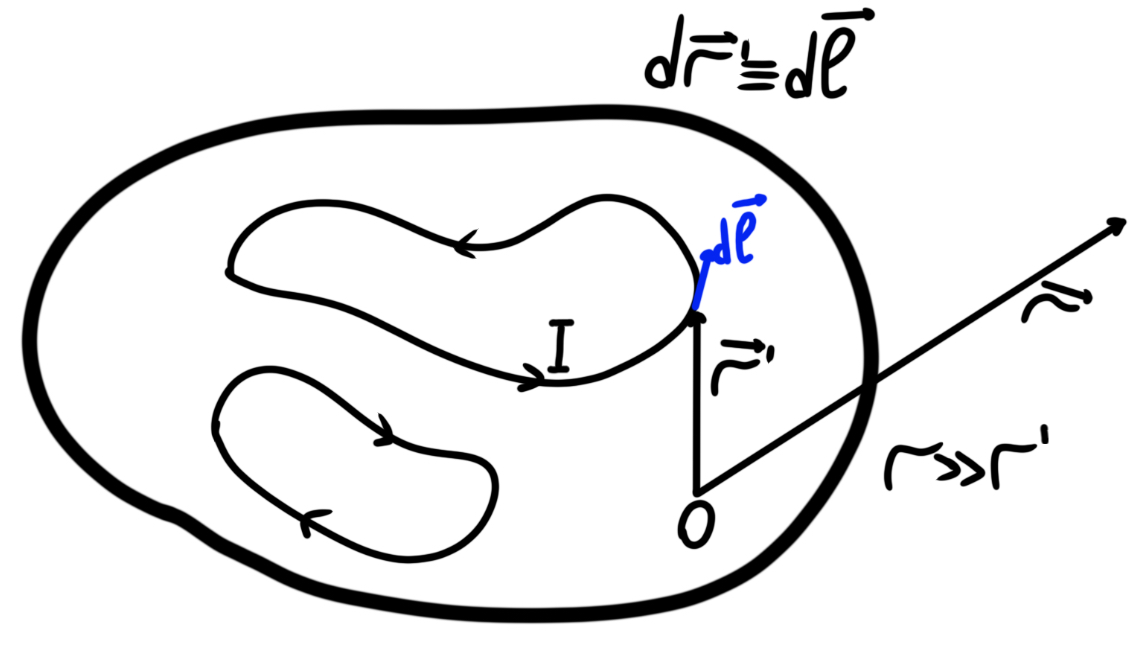
\includegraphics[width=0.5\textwidth]{im/69.png}
\end{center}

\begin{gather*}
    \vec{A}=\frac{q}{c} \iiint \frac{\vec{j}(\vec{r'})}{|\vec{r}-\vec{r'}|}dV'=\sum \frac{I}{c}\oint \frac{1}{|\vec{r}-\vec{r'}|}d\vec{r'} \\
    \text{в дальнейших формулах не будем писать }\Sigma \\
    \vec{j}dV'\rightarrow Id\vec{l}=Id\vec{r'} 
\end{gather*}

Вспомним разложение:

\[
\frac{1}{|\vec{r}-\vec{r'}|} =\frac{1}{r}+\frac{\vec{r}\cdot\vec{r'}}{r^3}+\dots (\text{ограничемся двумя членами})
\]

\begin{gather*}
    \vec{A}= \frac{I}{r}  \cancelto{0}{\oint \frac{1}{r}  d\vec{r'}}+ \frac{I}{cr^3} \oint (\vec{r}\vec{r'})d\vec{r'}= \\ 
    =\frac{I}{cr^3} \cancelto{0}{(\vec{r}\vec{r'})}\oint d\vec{r'}-\frac{I}{cr^3}\oint (\vec{r}d\vec{r'})\vec{r'}= \frac{I}{2cr^3} \oint \left[d\vec{r'}(\vec{r}\vec{r'})-\vec{r'}(\vec{r}d\vec{r'})\right] = \\
    =\frac{I}{2cr^3} \oint [\vec{r}\times [d \vec{r'}\times \vec{r}]]=\left[ \frac{\vec{r}}{r^3}\times \frac{I}{2c} \oint [d\vec{r'}\times \vec{r'}]   \right]= \frac{I}{2c} \oint \left[ [\vec{r}\times d\vec{r'}]\times \frac{\vec{r}}{r^3}  \right]      
\end{gather*}

\textit{Дипольный момент магнитного поля : }

\[
\boxed{\vec{m}\overset{df}{=} \sum \frac{I}{2c} \oint [\vec{r'}\times d\vec{r'}] }
\]

Веторный потенциал через магнитный диполь:

\[
\vec{A}=\frac{[\vec{m}\times \vec{r}]}{r^3} 
\]

Пусть есть один  плоский контур с током $I$:

\begin{minipage}[c]{0.5\textwidth} % Левая часть: изображение
    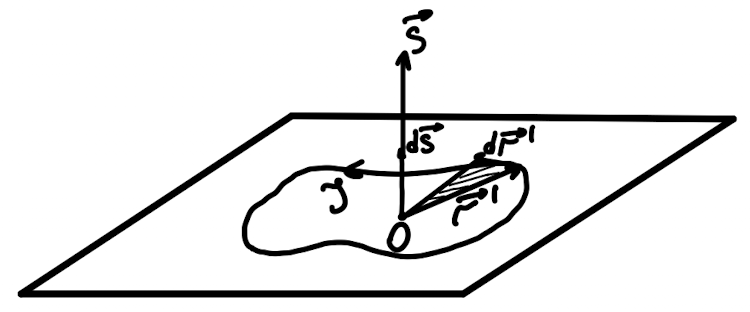
\includegraphics[width=\textwidth]{im/70.png} % Ваше изображение
\end{minipage}%
\hfill
\begin{minipage}[c]{0.55\textwidth} % Правая часть: текст
    \begin{gather*}
        \vec{m}=\frac{I}{2c} \oint [\vec{r'}\times d \vec{r'}]=\frac{I}{c} \int d\vec{S}= \frac{I}{c} \vec{S} \\
        \vec{m}= \frac{I}{c} \vec{S}
    \end{gather*}
\end{minipage}

Для распредленных токов $Id\vec{r'}\rightarrow \vec{j}\vec{r'}dV'$ и :

\[
\vec{m} =\frac{I}{2c} \iiint [\vec{r'}\times \vec{j}(\vec{r'})]dV' 
\]

\subsection*{Магнитное поле диполя}

\begin{gather*}
    \vec{H}=\mathrm{rot}\vec{A}=[\grad \times \left[ \vec{m}\times \frac{\vec{r}}{r^3} \right] ] = \vec{m} \overset{\overset{0}{    \rotatebox{90}{=}}}{\left( \grad \frac{r}{r^3}  \right)} -\overset{\downarrow}{\frac{\vec{r}}{r^3}}(\grad\vec{m})= \\
    =-(\vec{m}\grad)\frac{\vec{r}}{r^3}=-\vec{r}(\vec{m}\grad \frac{1}{r^3} )-\frac{1}{r^3}(\vec{m}\grad)\vec{r} \fbox{=}  \\
    \text{Вспомним :} \\
    \grad\vec{r}\frac{1}{r^3}=\frac{1}{r^3}\grad\vec{r}+ \vec{r}\grad \frac{1}{r^3}=\frac{3}{r^3}+\vec{r}\left( -\frac{3}{r^4} \grad r  \right)= \frac{3}{r^3}-\frac{3}{r^4}\frac{\vec{r}\vec{r}}{r}=0 \\
    \grad \frac{1}{r^3}=- \frac{3\vec{r}}{r^5} \\
    \fbox{=} -\frac{\vec{m}}{r^3}+ \frac{3(\vec{m}\vec{r})\vec{r}}{r^5}  
\end{gather*}

\[
\boxed{\vec{H}=-\frac{\vec{m}}{r^3}+ \frac{3(\vec{m}\vec{r})\vec{r}}{r^5} }
\]

